\chapter{Diffusive Shock Acceleration} \label{A3_DSA}

At Earth, the energy spectrum of cosmic rays have been measured up to $10^{20}\,\eV$ (see \autoref{sec:chapter_1_cr_spectrum}). But how do cosmic rays reach these enormous energies? Fermi, in 1949, proposed a mechanism where cosmic rays are accelerated through the interaction with magnetic field irregularities in ISM gas clouds \citep{1949PhRv...75.1169F}. However, the amount of energy gained through these interactions is relatively small to explain the highest energy cosmic rays observed at Earth. Fermi's original theory was modified in the 1970s to consider the acceleration of cosmic rays as they travel through a shock wave generated by, for example, a SNR \citep{1977DoSSR.234.1306K,1977ICRC...11..132A,1978MNRAS.182..147B,1978MNRAS.182..443B,1978ApJ...221L..29B}. This is known as diffusive shock acceleration.

\section{Fermi's Original Theory}

In Fermi's original theory, a cosmic ray with energy $E_1$  scatters of a ISM gas cloud (travelling at velocity $v_c$ in the lab frame) at angle $\theta_1$ (see \autoref{fig:A3_DSA_fermi_orig_frames}) and exits the cloud with energy $E_2$ and angle $\theta_2$. Using Lorentz transformations, the original energy in the cloud frame (primed frame) is given by:

\begin{figure}[h!]
    \centering
    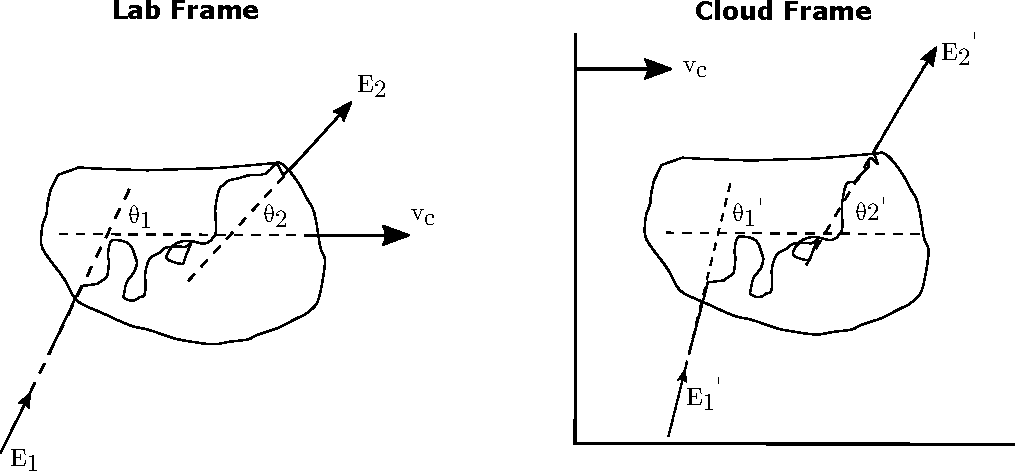
\includegraphics{A3_Diffusive_Shock_Acceleration/Images/fermi_original_theory_frames.pdf}
    \caption{In the lab frame (\textit{left}), a cosmic ray with energy $E_1$ enters an ISM cloud (travelling at speed $v_c$) at angle $\theta_1$ and scatters off magnetic field turbulence and exits the cloud with energy $E_2$ and angle $\theta_2$. The same process is shown in the right, but in the reference frame of the cloud (labeled as primed).}
    \label{fig:A3_DSA_fermi_orig_frames}
\end{figure}

\begin{equation}
    \begin{aligned}
        E_1'=\gamma_cE_1\qty(1-\beta_c\cos\theta_1)\text{ ,}
    \end{aligned}
\end{equation}
\noindent where $\beta_c=v_c/c$ and $\gamma_c=1/\sqrt{1-\beta_c^2}$. The scattering is collisionless (elastic) in the reference frame of the cloud, giving $E_1'=E_2'$. The final energy in the lab frame is then:

\begin{equation}
    \begin{aligned}
        E_2&=\gamma_c E_2'\qty(1+\beta_c\cos\theta_2') \\
        &=\gamma_c^2E_1\qty(1+\beta_c\cos\theta_2')\qty(1-\beta_c\cos\theta_1) \text{ ,}
    \end{aligned}
\end{equation}
\noindent giving the cosmic-ray fractional energy gain to be:

\begin{equation}
    \begin{aligned}
        \frac{\Delta E}{E}&=\frac{E_2-E_1}{E_1} \\
        &=\frac{1-\beta_c\cos\theta_1+\beta_c\cos\theta_1+\beta_c^2\cos\theta_1\cos\theta_2'}{\qty(1-\beta_c^2)}-1\text{ .}
    \end{aligned} \label{eq:A3_DSA_fermi_orig_frac_energy}
\end{equation}
\noindent Considering the average fractional energy gain ($\langle \Delta E/E \rangle$), the outgoing direction of the cosmic ray in the clouds reference frame is randomised. Therefore, $\langle \cos\theta_2'=0 \rangle$. To calculate the average original cosmic-ray angle ($\langle \cos\theta_1 \rangle$), consider the ISM cloud traveling a distance $v_ct$ in a `sea' of cosmic rays travelling at speed $v_\text{CR}$ (see \autoref{fig:A3_fermi_origin_theta1}). In time $t$, all cosmic rays in length $L$ will enter the cloud. For relativistic cosmic rays ($v_\text{cr}>>v_c$),
\begin{SCfigure}[2.3][b!]
    \centering
    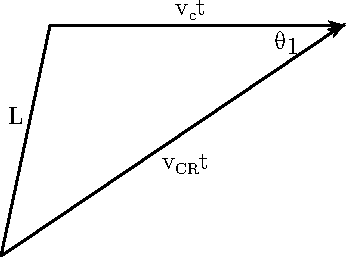
\includegraphics[width=0.3\textwidth]{A3_Diffusive_Shock_Acceleration/Images/fermi_original_theta1.pdf}
    \caption{A ISM cloud travelling at speed $v_c$ in a `sea' of cosmic rays. In time $t$, the cosmic rays in path $L$ with speed $v_\text{CR}$ will enter the cloud.}
    \label{fig:A3_fermi_origin_theta1}
\end{SCfigure}
\begin{equation}
    \begin{aligned}
        L&=t\sqrt{v_\text{CR}^2+v_c^2-2v_\text{CR}v_c\cos\theta_1} \\
        &\approx t\qty(v_\text{CR}-v_c\cos\theta_1) \text{ .}
    \end{aligned}
\end{equation}
\noindent For a spherical cloud of radius $r$ and cross-section $\sigma=\pi r^2$, the collision rate, $R$, is:

\begin{equation}
    \begin{aligned}
        R&=\frac{n_\text{CR}L\sigma}{t} \\
        &=n_\text{CR}\sigma\qty(v_\text{CR}-v_c\cos\theta_1) \text { ,}
    \end{aligned}
\end{equation}
\noindent where $n_\text{CR}$ is the cosmic-ray density. For an isotropic cosmic-ray distribution, $\dd{n_\text{CR}}/\dd{\cos\theta_1}=n_\text{CR}/2$ for $-1<\cos\theta_1<1$, the collision rate is described by:

\begin{equation}
    \begin{aligned}
        R&=\frac{n_\text{CR}L\sigma}{t} \\
        &=\frac{n_\text{CR}\sigma}{2}\int_{-1}^1\dd{\cos\theta_1}\qty(v_\text{CR}-v_c\cos\theta_1) \text{ .}
    \end{aligned}
\end{equation}
\noindent giving the probability distribution of collision at angle $\theta_1$ to be $p_\text{coll}\propto \qty(1-\beta_c)$ for relativistic cosmic rays. The average value of $\cos\theta_1$ is then:

\begin{equation}
    \begin{aligned}
        \langle \cos\theta_1\rangle &=\frac{\int_{-1}^1\dd{\cos\theta_1}p_\text{coll}\cos\theta_1}{\int_{-1}^1\dd{\cos\theta_1}p_\text{coll}} \\
        &=-\frac{\beta}{3} \text{ .}
    \end{aligned} \label{eq:A3_DSA_fermi_orig_av_theta1}
\end{equation} 
\noindent Combining \autoref{eq:A3_DSA_fermi_orig_frac_energy}, \autoref{eq:A3_DSA_fermi_orig_av_theta1} and that $\langle \cos\theta_2' \rangle=0$:

\begin{equation}
    \begin{aligned}
        \langle \frac{\Delta E}{E} \rangle&=\frac{1-\beta_c\langle\cos\theta_1\rangle+\beta_c\cos\langle\theta_1\rangle+\beta_c^2\langle\cos\theta_1\rangle\langle\cos\theta_2'\rangle}{\qty(1-\beta_c^2)} \\
        &= \frac{4}{3}\beta_c^2 \text{ .}
    \end{aligned}
\end{equation}
\noindent The average fractional energy gain is positive and second-order in $\beta_c$ (Fermi's original theory is also known as second-order Fermi acceleration). ISM gas clouds have velocity $\approx 15\,\kmpersec$, resulting in a small fractional energy gain that cannot explain the highest energy cosmic rays observed at Earth. \citep{1949PhRv...75.1169F}. 

\section{Diffusive Shock Acceleration}

Diffusive shock acceleration is a modified version of Fermi's original theory that considers acceleration at a shock front (e.g. SNR shock). The shock travels at velocity $v_s$ in the upsream reference frame (the region of ISM that has not been `shocked') with a ISM gas cloud downstream of the shock having velocity $v_c$ (see \autoref{fig:A3_shock_dynamics2}). In the reference frame of the shock, the material upstream of the shock travels towards the shock at velocity $U_1=v_s$ and the downstream cloud now has velcoity $U_2=v_s-v_c$. The compression ratio is defined to be the mass density ratio of the shocked and unshocked material:

\begin{equation}
    \begin{aligned}
        r&=\frac{\rho_2}{\rho_1}\text{ ,}
    \end{aligned}
\end{equation}
\noindent where $\rho_1$ and $\rho_2$ are the densities upstream and downstream of the shock respectively. From conservation of mass:

\begin{equation}
    \begin{aligned}
        \rho_1U_{1}&=\rho_2U_2=A \\
        \therefore U_{1}&=rU_{2}\text{ ,}
    \end{aligned} \label{eq:A3_velocity_ratios}
\end{equation}
\noindent where $A$ is a constant. From conservation of momentum:
\begin{figure}[!b]
	\centering
	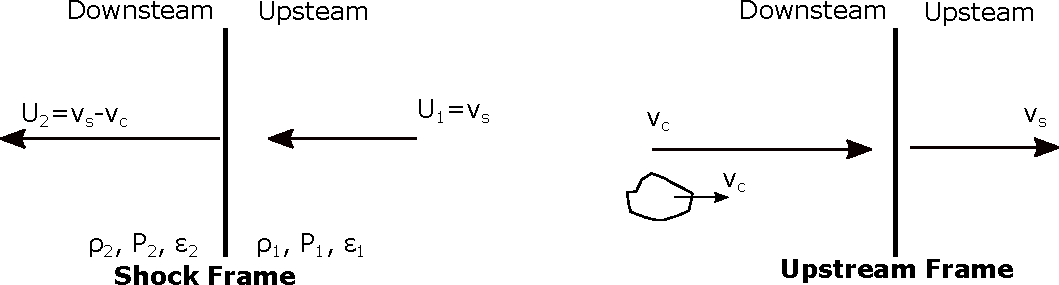
\includegraphics[width=1.0\textwidth]{A3_Diffusive_Shock_Acceleration/Images/upstream_downstream.pdf}
	\caption{A shock travelling through the ISM with velocity $v_s$ in the upstream reference frame. (\textit{left}) In the reference frame of the shock, the material upstream travels towards the shock at velocity $U_1=v_s$. The material downstream of the shock travels at velocity $U_2=v_s-v_c$, where $v_c$ is the velocity of an ISM gas cloud in the upstream reference frame (\textit{right}). The material upstream and downstream of the shock have densities, pressure and internal energy $\rho$, $P$ and $\epsilon$ respectively.}
	\label{fig:A3_shock_dynamics2}
\end{figure}
\begin{subequations}
    \begin{alignat}{1}
        AU_{1}&=AU_{2}+P_2\text{ ,}
    \end{alignat} \label{eq:A3_dsa_momentum_cons}
\end{subequations}
\noindent with $P_2$ being the pressure downstream. From the conservation of energy:
\begin{equation}
    \begin{aligned}
        \frac{1}{2}AU_{1}^2&=\frac{1}{2}U_{2}^2+U_{2}\qty(\epsilon_2+P_2)\text{ ,}
    \end{aligned} \label{eq:A3_DSA_energy_cons}
\end{equation}
\noindent where $\epsilon_2$ is the downstream internal energy. Combining \autoref{eq:A3_velocity_ratios}, \autoref{eq:A3_dsa_momentum_cons} and \autoref{eq:A3_DSA_energy_cons} gives the compression ratio to be:

\begin{equation}
    \begin{aligned}
        r&=1+\frac{2\epsilon_2}{P_2}\text{ ,}
    \end{aligned}
\end{equation}
\noindent and $r$ takes values $4$ and $7$ for monatomic non-relativistic and relativistic gas respectively  \citep{1983RPPh...46..973D}.
\newpar 
From \autoref{eq:A3_velocity_ratios}, the velocity of the downstream material (in the shock reference frame) can be expressed in terms of the compression ratio:

\begin{equation}
    \begin{aligned}
        v_c &=v_s-U_2=v_s-\frac{v_s}{r} \\
        \therefore \frac{v_c}{v_s}&=\frac{r-1}{r}\text{ ,}
    \end{aligned} \label{eq:down_upstream_v_ratio}
\end{equation}
\noindent For non-relativistic particles ${v_c}/{v_s}=3/4$.
\begin{SCfigure}[0.5][h]
	\centering
	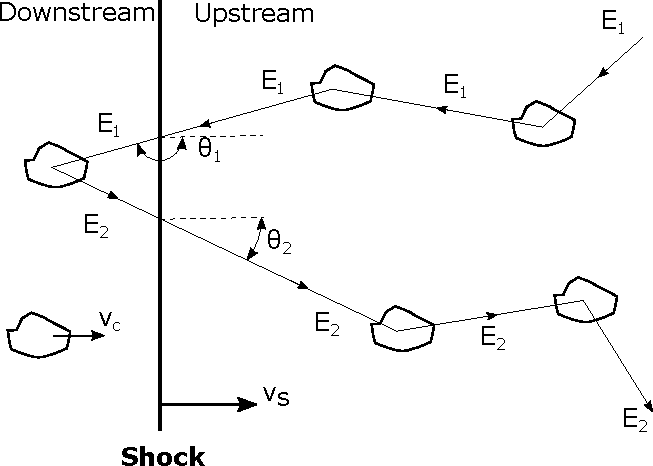
\includegraphics[width=0.65\textwidth]{A3_Diffusive_Shock_Acceleration/Images/dsa.pdf}
	\caption{Aa cosmic ray of energy $E_1$ travels upstream to downstream of the shock with no change of energy. The cosmic ray scatters off magnetic field tubulence in a cloud downstream of the shock and passes back upstream of the shock with energy $E_2$. This process can repeat or the cosmic ray can escape the system.}
	\label{fig:A3_shock_dynamics3}
\end{SCfigure}
\newpar 
Now consider the scenario shown in \autoref{fig:A3_shock_dynamics3}, where a cosmic ray of energy $E_1$, velocity $v_\text{CR}$ and angle $\theta_1$ travels upstream to downstream of the shock and scatters off a ISM cloud travelling at velocity $U_2'$. The cosmic ray, with energy $E_2$, travels back upstream at angle $\theta_2$. The rate that cosmic rays travel upstream to downstream ($u\rightarrow d$) and downstream to upstream ($d\rightarrow u$) is given by:


\begin{alignat}{2}
    R_{u\rightarrow d}\qty(\theta_1)&\approx-n_\text{CR}v_\text{CR}\cos\theta_1,\quad &\ang{90}<\theta_1<\ang{180} \label{eq:ASA_DSA_rate_ud} \\
    R_{d\rightarrow u}\qty(\theta_2')&\approx n_\text{CR}v_\text{CR}\cos\theta_2'\quad&\ang{0}<\theta_2<\ang{90} \text{ ,}
\end{alignat}
\noindent giving the probability of crossings to be:

\begin{equation}
    \begin{aligned}
        p_{u\rightarrow d}\qty(\theta_1)&\propto -\cos\theta_1 \\
        p_{d\rightarrow u}\qty(\theta_1)&\propto \cos\theta_2'  \text{ .}
    \end{aligned}
\end{equation}
\noindent Therefore, the average values of $\cos\theta_1$ and $\cos\theta_2'$ are:

\begin{equation}
    \begin{aligned}
    \expectation{\cos\theta_1}&=\frac{\int_{-1}^{0} \cos\theta_1^2\dd{\cos\theta_1}}{\int_{-1}^{0}\cos\theta_1 \dd{\cos\theta_1}}=-\frac{2}{3} \\
    \expectation{\cos\theta_2'}&=\frac{\int_{0}^{1} {\cos\theta_2'}^2\dd{\cos\theta_2'}}{\int_{0}^{1}\cos\theta_2' \dd{\cos\theta_2'}}=\frac{2}{3}\text{ .}
    \end{aligned} \label{eq:A3_DSA_fermi_second_angle}
\end{equation}

\noindent Combining \autoref{eq:A3_DSA_fermi_orig_frac_energy} and \autoref{eq:A3_DSA_fermi_second_angle} gives the average fractional energy gain:

\begin{equation}
    \begin{aligned}
    \expectation{\frac{\Delta E}{E}}
	&=\frac{\beta^2+\frac{4}{3}\beta+\frac{4}{9}\beta^2}{1-\beta_\text{cloud}^2}\text{ ,}
    \end{aligned} 
\end{equation}
\noindent where $\beta_c=v_c/c$. For $\beta_c\ll 1$:

\begin{equation}
    \begin{aligned}
    \expectation{\frac{\Delta E}{E}}
	&\approx \frac{4}{3}\beta 
    \end{aligned} 
\end{equation}
\noindent Each time the cosmic ray travels back and across the shock, the cosmic ray has increased its energy by a factor $v_s/c$, where $v_s\approx 10^4\,\kmpersec$ for SNR shocks Therefore, diffusive shock acceleration is far more efficient than Fermi's original theory in accelerating cosmic rays.  Diffusive shock acceleration is also known as first-order Fermi acceleration as the average energy gain is first order with $\beta_c$. 

\subsection{Cosmic-Ray Energy Spectrum}

To calculate the energy spectrum of cosmic rays accelerated by diffusive shock acceleration, the probability of the cosmic ray escaping to the the shock must be calculated. The probability of escape is the ratio of the rate that cosmic rays are lost downstream and the total rate that cosmic rays cross the shock upstream to downstream ($p_\text{esc}=R_\text{loss}/R_{tot}$). The rate that cosmic rays are lost downstream is:

\begin{equation}
    \begin{aligned}
        R_\text{loss}&=n_\text{CR}U_2=n_\text{CR}\frac{v_s}{r}\text{ ,}
    \end{aligned}
\end{equation}
\noindent and the total rate that cosmic rays travel upstream to downstream can be obtained by integrating \autoref{eq:ASA_DSA_rate_ud} over all possible angles:

\begin{equation}
    \begin{aligned}
        R_{tot}&=\frac{1}{4\pi}\int_{-1}^0\dd{\cos\theta_1}2\pi R_{u\rightarrow d}\qty(\cos\theta_1) \\
        &=\frac{n_\text{CR}v_\text{CR}}{4} \text{ .}
    \end{aligned}
\end{equation}
\noindent This gives the probability of escape:

\begin{equation}
    \begin{aligned}
        p_\text{esc}&=\frac{4v_s}{rv_\text{CR}} \text{ .}
    \end{aligned}
\end{equation}
\noindent The integrated energy spectrum, $N\qty(>E)$ is proportional to the probability that a cosmic ray returns to the shock after $k$ crossings:

\begin{equation}
    \begin{aligned}
        N\qty(>E)\propto p_\text{ret}&=\qty(1-p_\text{esc})^k \text{ ,}
    \end{aligned}
\end{equation}
\noindent where the cosmic ray has energy:

\begin{equation}
    \begin{aligned}
        E_k&=E_0\qty(1+\frac{\Delta E}{E})^k \\
        \therefore k&=\frac{\ln(E/E_0)}{\ln(1+\Delta E/E)}
    \end{aligned}
\end{equation}
\noindent with $E_0$ being the original cosmic-ray energy. Giving:

\begin{equation}
    \begin{aligned}
        N\qty(>E)&=C\qty(1-\frac{4v_s}{rv_\text{CR}})^k \text{ ,}
    \end{aligned}
\end{equation}
\noindent where $C$ is a constant. The integrated energy spectrum can be expressed in terms of a power-law, $N\qty(>E)=AE^{-\Gamma}$, with:

\begin{equation}
    \begin{aligned}
        \Gamma = -\frac{\ln(1-\frac{4v_s}{rv_\text{CR}})}{\ln(1+\frac{4v_s\qty(r-1)}{3rc})} \text{ .}
    \end{aligned}
\end{equation}
\noindent For non-relativistic shocks such as a SNR ($v_s\ll c$),  $\Gamma\approx 3/\qty(r-1)$. The differential energy spectrum becomes:

\begin{equation}
    \begin{aligned}
        \dv{N}{E}\propto E^{-({r+2})/({r-1})} \text{ .}
    \end{aligned}
\end{equation}
\noindent For strong shocks, $r=4$, the differential energy spectrum takes form $\dv{N}{E}\propto E^{-2}$.